%\documentclass[12pt, draftclsnofoot, onecolumn,letterpaper]{IEEEtran}
\documentclass[12pt, letterpaper]{article}
%\documentclass[12pt, letterpaper]{IEEEtran}
\usepackage{ multirow }
\usepackage{longtable}
\usepackage{geometry}
\usepackage{ragged2e}
\usepackage[table]{xcolor}
\usepackage{booktabs}
\usepackage{graphicx}
\usepackage{caption}
\usepackage{subcaption}
\usepackage{lipsum}
\usepackage{makeidx}
\usepackage{enumerate}
\usepackage{color}
\usepackage{refstyle}
\usepackage{cite}
\usepackage{amsmath}
\usepackage{amssymb}
\usepackage{nomencl}
\usepackage{amsmath}
\usepackage{multirow}
\usepackage{graphicx}
\usepackage{multirow}
\usepackage{anysize}
\usepackage{float}
\usepackage{epstopdf}
\usepackage{threeparttable}
\usepackage{multicol}
\usepackage{amssymb}
\usepackage{adjustbox}
%\usepackage[none]{hyphenat}
%\usepackage{float}

%\usepackage{fixltx2e}
\usepackage{amsmath, amssymb, upgreek, amsthm}
\usepackage{graphicx}
\usepackage{tikz}
\geometry{letterpaper, left=20mm, right=20mm, top=20mm, bottom=20mm}
\usetikzlibrary{patterns} % LATEX and plain TEX when using Tik Z
\allowdisplaybreaks
\setlength{\textfloatsep}{2ex}
\usepackage{array}
\usepackage{enumitem}
\setlength{\parindent}{1 em}
\setlength{\parskip}{0.5 em}
\renewcommand{\baselinestretch}{1.25}
\def\dsd{d_\text{SD}}
\def\Rcoop{R_\text{Coop}}
\def\rhd{R_\text{HD}}
\def\rsd{R_\text{SD}}
\def\rsh{R_\text{SH}}
\def\Pcoops{\mathcal{P}^\text{Succ}_\text{Coop}}
\def\dsh{d_\text{SH}}
\def\dhd{d_\text{HD}}
\def\psibar{\overline{\mathcal{P}}^\text{Succ}_{i}}
\def\psbara{\overline{\mathcal{P}}^\text{Succ}_{1}}
\def\psbarb{\overline{\mathcal{P}}^\text{Succ}_{2}}
\def\psbarc{\overline{\mathcal{P}}^\text{Succ}_{3}}
\def\psbard{\overline{\mathcal{P}}^\text{Succ}_{4}}
\def\psbare{\overline{\mathcal{P}}^\text{Succ}_{5}}
\def\Ri{R_{i}}
\def\Ps{\mathcal{P}^\text{Succ}_\text{Direct}}
\def\frk{\mathrm{f}_{r_k}(r)}
\def\Rcoopj{R_\text{coop}^j}
\title{\bf \vspace*{-4ex} Statement of Responses to the Editor and the Reviewers of Paper-TCOM-TPS-19-0363.R1 \\[-6ex]}
\date{}

\begin{document}
%\vspace*{-10ex}
%\sloppy
\maketitle
We would like to thank the editor and reviewers for their comments on our manuscript.
We hope that the modifications that we have made to the manuscript, and the responses that we have
provided herein will alleviate the reviewers' concerns. Below, please find our detailed responses to the editor and reviewers' comments and suggestions.
\\ [-3.ex]
% % % % % % % % % % % % % % % Editor % % % % % % % % % % % % % % % % % % % %


\clearpage
\noindent
\begin{longtable}{|p{0.975\textwidth}|}
\hline \hline
\Centering
\cellcolor{gray!60}
\textbf{Editor} \\
\hline \hline %\hline \hline \hline
\RaggedRight
\cellcolor{gray!15}
\textbf{\noindent Comment1:} ``In particular, in agreement with the reviewers, the paper would greatly benefit from a clearer focus with respect to the applicability of the discussed model specifically for nanomachines. What are the intended nanomachines? How will they be realized and what is their applicability within a synaptic cleft? How will they be implanted? A revised focus is suggested if sufficient clarity in these directions cannot be reached.''\\
\hline
\end{longtable}

\vspace*{-1\baselineskip}
\noindent \textbf{Response:\\}
We would like to thank the editor for his comment on our manuscript. According to the advances in nano-technology and nano-communications, different design strategies for intelligent nano-devices interfaced with the neuronal tissue were proposed in the literature. The proposed system model in this manuscript is based on one of them. We clarify more about this issue in the following. We refer to the following list of references in our explanation in this comment:

\begin{longtable}{|p{0.975\textwidth}|}
\hline \hline
\RaggedRight
\cellcolor{green!10}
[1] F. Patolsky, B. P. Timko, G. Yu, Y. Fang, A. B. Greytak, G. Zheng, and C. M. Lieber, ``Detection, stimulation, and inhibition of neuronal signals with high-density nanowire transistor arrays,'' Science, vol. 313, no. 5790, pp. 1100-1104, 2006.

[2] N. Sakai, J. Mareda, and S. Matile, ``Ion channels and pores, made from scratch,'' Molecular BioSyst., vol. 3, pp. 658-666, 2007.

[3] P. Gorostiza and E. Isacoff, ``Optical switches and triggers for the manipulation of ion channels and pores,'' Molecular BioSyst., vol. 3, pp. 686-704, 2007.

[4] Mesiti, Fabio, and Ilangko Balasingham. ``Nanomachine-to-neuron communication interfaces for neuronal stimulation at nanoscale.'', IEEE Journal on Selected Areas in Communications, vol. 31, no. 12, pp. 695-704, 2013.

[5] N. Rouach, E. Avignone, W. Même, A. Koulakoff, L. Venance, F. Blomstrand, and C. Giaume, ``Gap junctions and connexin expression in the normal and pathological central nervous system,'' Biology Cell, vol. 94, no. 7-8, pp. 457-475, 2002.

[6] J. Hjorth, K. T. Blackwell, and J. Hellgren Kotaleski, ``Gap junctions between striatal fast-spiking interneurons regulate spiking activity and synchronization as a function of cortical activity'', J. Neuroscience, vol. 29, no. 16, pp. 5276-5286, 2009.

[7] R. D. Traub, M. A. Whittington, E. H. Buhl, F. E. N. LeBeau, A. Bibbig, S. Boyd, H. Cross, and T. Baldeweg, ``A possible role for gap junctions in generation of very fast EEG oscillations preceding the onset of, and perhaps initiating, seizures,'' Epilepsia, vol. 42, no. 2, pp. 153-170, 2001.
\\
\hline
\end{longtable}


\clearpage
In [1], the authors described the successful attempt to interface nano-wire (NW) FET transistors (SiNW-neurons) with soma, dendrites and axon, allowing high precision measurement and
stimulation with an array of 50 NW connections per neuron. The synthesis of ion channels and pores, assembled artificially by chemical composition were reported in [2], whereas synthetic nano-scale actuators (nano-toggles, nano-keys and nano-tweezers) to manipulate ion channels were proposed in [3].
Hence, the advances in the molecular manipulation of the matter can allow the fabrication of bio-inspired SnM interfaces.
Upon these considerations and the available nano-technology, the authors in [4] identified a set of possible SnM interface implementations. We employed one type of these interfaces in our system model according to [4] which is denoted as Gap Junction Interface.


\textbf{Gap Junction Interface [4]}:

With gap junctions, two cellular membranes in direct contact are separated by only 3 nm and for each side, clusters of \textit{connexine} (Cx36) proteins [5], combine to form a channel with diameter 1-2 nm, the \textit{connexine}, allowing bidirectional flows of ions (currents) between cells. Synthetic connexines assembled \textit{in-situ} by SnMs could allow the opening of additional ion channels on the membrane, enhancing the neuronal activity. In the following figure [4], a sample scenario with multiple SnMs attached to the target neuron is depicted. This method is motivated and supported by neuro-scientific studies [6], [7] reporting the important role of gap junctions in \textit{oscillatory behaviors} and \textit{synchronization} phenomena between neurons.

\begin{figure}[H]
\centering
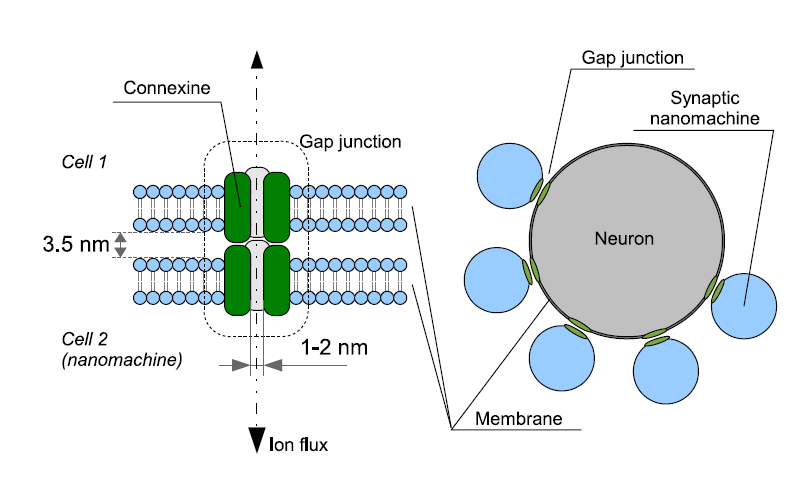
\includegraphics[width=.78\textwidth,height=.3\textheight]{Gap.png}
\caption{ Diagram of a SnM based on gap junctions. The neuronal membrane is in contact with each SnM, establishing additional connexone channels which allow the flow of ions and currents [4].}
\label{new_1}
\end{figure}








% % % % % % % % % % % % % % % Reviewer 1 % % % % % % % % % % % % % % % % % % % %
\clearpage
\noindent
\begin{longtable}{|p{.975\textwidth}|}
\hline \hline %\hline \hline \hline
\Centering
\cellcolor{gray!60}
\textbf{Reviewer 1} \\
\hline \hline %\hline \hline \hline
\RaggedRight
\cellcolor{gray!15}
\textbf{\noindent Comment1:} ``I thank the authors for providing a modified paper. The authors have made changes in the previous system model that struck this reviewer as the biggest limitation of the paper. The novel described solution in Figure 1 does make more sense compared to the previous one.''\\
\hline
\end{longtable}
\vspace*{-1\baselineskip}
\noindent \textbf{Response:\\}
We would like to thank the reviewer for careful and thorough reading of this manuscript and for the thoughtful and positive comments and constructive suggestions, which helped us to improve the quality of this manuscript. We hope that the responses provided herein can alleviate the reviewer concerns.





\begin{longtable}{|p{0.975\textwidth}|}
\hline \hline
\RaggedRight
\cellcolor{gray!15}
\textbf{\noindent Comment 2:} ``However, the scaling problem arises now. The synaptic channel/cleft between \textbf{Tx} and \textbf{Rx} is very narrow (tens of nm). If the authors suggest nano-machines, e.g., as in the scenario shown in Figure 2 (c), both nano-machines are envisioned to co-locate in the cleft, 3 nm distant from the synaptic terminals. What is the size of nano-machines then? How realistic is that owing to the complexity of these nano-machines? Wouldn't it be much easier to consider artificial synapse instead?''\\
\hline
\end{longtable}
\vspace*{-1\baselineskip}
\noindent \textbf{Response:\\}
According to the advances in nano-technology and nano-communications, different design strategies for intelligent nano-devices interfaced with the neuronal tissue were proposed in the literature. The proposed system model in this manuscript is based on one of them.
In the proposed system model, we need to consider the assumptions of real synapses since the real neurons play the role of \textbf{Tx} and \textbf{Rx} in the most of scenarios while in the artificial synapses, the assumptions are different.

About the scaling problem, the width of synaptic cleft is about tens of nm and in the worth case scenario where nano-machines are located in both terminals, 6 nm is required for SnM interfaces. Hence, there is sufficient room for nano-machines since they are much smaller than the neurons. In addition, some references in the literature discussed about the implementation of these interfaces.
We clarified about this issue in the following:

\clearpage
We refer to the following list of references in our explanation in this comment:

\begin{longtable}{|p{0.975\textwidth}|}
\hline \hline
\RaggedRight
\cellcolor{green!10}
[1] F. Patolsky, B. P. Timko, G. Yu, Y. Fang, A. B. Greytak, G. Zheng, and C. M. Lieber, ``Detection, stimulation, and inhibition of neuronal signals with high-density nanowire transistor arrays,'' Science, vol. 313, no. 5790, pp. 1100-1104, 2006.

[2] N. Sakai, J. Mareda, and S. Matile, ``Ion channels and pores, made from scratch,'' Molecular BioSyst., vol. 3, pp. 658-666, 2007.

[3] P. Gorostiza and E. Isacoff, ``Optical switches and triggers for the manipulation of ion channels and pores,'' Molecular BioSyst., vol. 3, pp. 686-704, 2007.

[4] Mesiti, Fabio, and Ilangko Balasingham. ``Nanomachine-to-neuron communication interfaces for neuronal stimulation at nanoscale.'', IEEE Journal on Selected Areas in Communications, vol. 31, no. 12, pp. 695-704, 2013.

[5] N. Rouach, E. Avignone, W. Même, A. Koulakoff, L. Venance, F. Blomstrand, and C. Giaume, ``Gap junctions and connexin expression in the normal and pathological central nervous system,'' Biology Cell, vol. 94, no. 7-8, pp. 457-475, 2002.

[6] J. Hjorth, K. T. Blackwell, and J. Hellgren Kotaleski, ``Gap junctions between striatal fast-spiking interneurons regulate spiking activity and synchronization as a function of cortical activity'', J. Neuroscience, vol. 29, no. 16, pp. 5276-5286, 2009.

[7] R. D. Traub, M. A. Whittington, E. H. Buhl, F. E. N. LeBeau, A. Bibbig, S. Boyd, H. Cross, and T. Baldeweg, ``A possible role for gap junctions in generation of very fast EEG oscillations preceding the onset of, and perhaps initiating, seizures,'' Epilepsia, vol. 42, no. 2, pp. 153-170, 2001.
\\
\hline
\end{longtable}


\clearpage
In [1], the authors described the successful attempt to interface nano-wire (NW) FET transistors (SiNW-neurons) with soma, dendrites and axon, allowing high precision measurement and
stimulation with an array of 50 NW connections per neuron. The synthesis of ion channels and pores, assembled artificially by chemical composition were reported in [2], whereas synthetic nano-scale actuators (nano-toggles, nano-keys and nano-tweezers) to manipulate ion channels were proposed in [3].
Hence, the advances in the molecular manipulation of the matter can allow the fabrication of bio-inspired SnM interfaces.
Upon these considerations and the available nano-technology, the authors in [4] identified a set of possible SnM interface implementations. We employed one type of these interfaces in our system model according to [4] which is denoted as Gap Junction Interface.


\textbf{Gap Junction Interface [4]}:

With gap junctions, two cellular membranes in direct contact are separated by only 3 nm and for each side, clusters of \textit{connexine} (Cx36) proteins [5], combine to form a channel with diameter 1-2 nm, the \textit{connexine}, allowing bidirectional flows of ions (currents) between cells. Synthetic connexines assembled \textit{in-situ} by SnMs could allow the opening of additional ion channels on the membrane, enhancing the neuronal activity. In the following figure [4], a sample scenario with multiple SnMs attached to the target neuron is depicted. This method is motivated and supported by neuro-scientific studies [6], [7] reporting the important role of gap junctions in \textit{oscillatory behaviors} and \textit{synchronization} phenomena between neurons.

\begin{figure}[H]
\centering
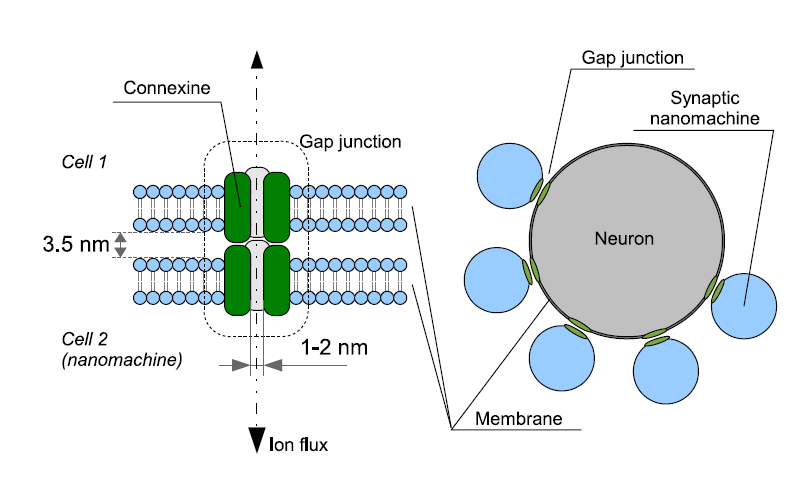
\includegraphics[width=.78\textwidth,height=.3\textheight]{Gap.png}
\caption{ Diagram of a SnM based on gap junctions. The neuronal membrane is in contact with each SnM, establishing additional connexone channels which allow the flow of ions and currents [4].}
\label{new_1}
\end{figure}




%%%%%%%%%%%%%%%%%%%%%%%%%%%%%%%%%%%%%%%%%%%%%%%%%%%%%%%%

\clearpage
\noindent
\begin{longtable}{|p{0.975\textwidth}|}
\hline \hline
\Centering
\cellcolor{gray!45}
\textbf{Reviewer 2} \\
\hline \hline
\RaggedRight
\cellcolor{gray!15}
\textbf{\noindent Comment 1:} ``The paper has been improved according to the previous comments from this reviewer and only the following minor issues have remained.''\\
\hline
\end{longtable}
\vspace*{-1\baselineskip}
\noindent \textbf{Response:\\}
We would like to thank the reviewer for careful and thorough reading of this manuscript and
for the thoughtful comments and constructive suggestions, which help us to improve the quality of
this manuscript. We hope that the responses provided herein can alleviate the reviewer concerns.



\begin{longtable}{|p{0.975\textwidth}|}
\hline \hline
\RaggedRight
\cellcolor{gray!15}
\textbf{\noindent Comment 2:} ``In Introduction, page 5, ``We consider a neuro-spike communication channel between two neurons located in the motor cortex region of the brain where the information is encoded by spike time intervals.''.  Please provide a reference for this sentence.''\\
\hline
\end{longtable}
\vspace*{-1\baselineskip}
\noindent \textbf{Response:\\}
Neural coding refers to the mapping from the stimulus to the configurations of the generated
spikes by neurons. Neurons employ the spike rate coding and temporal coding to transmit information via action potentials. As we explained in the manuscript, none of the papers in the literature proposed a model for neuro-spike communication channel in the motor cortex region when temporal modulations
are employed to convey information. However, there are some papers that assumed temporal modulations in the motor cortex region. We referred to one of these papers in the new manuscript based on the reviewer comment as
\begin{longtable}{|p{0.975\textwidth}|}
\hline \hline
\RaggedRight
\cellcolor{green!10}
We consider a neuro-spike communication channel between two neurons located in the motor cortex region of the brain where the information is encoded by spike time intervals [30].
\\
\hline
\end{longtable}
The referred paper is
\begin{longtable}{|p{0.975\textwidth}|}
\hline \hline
\RaggedRight
\cellcolor{green!10}
[30] Hatsopoulos N, Geman S, Amarasingham A, Bienenstock E., ``At what time scale does the nervous system operate?'', Neurocomputing, vol. 1, no. 52, pp.25-29, 2003.
\\
\hline
\end{longtable}

\clearpage
\begin{longtable}{|p{0.975\textwidth}|}
\hline \hline
\RaggedRight
\cellcolor{gray!15}
\textbf{\noindent Comment 3:} ``In System Model, the possibility of placing nano-machines in synapses located between motor cortex neurons must be proved. This action needs invasive surgeries, which cause further damage to the neurons.''\\
\hline
\end{longtable}
\vspace*{-1\baselineskip}
\noindent \textbf{Response:\\}
According to the advances in nano-technology and nano-communications, different design strategies
for intelligent nano-devices interfaced with the neuronal tissue were proposed in the literature. The
proposed system model in this manuscript is based on one of them. We clarify more about this issue in the following.
We refer to the following list of references in our explanation in this comment:

\begin{longtable}{|p{0.975\textwidth}|}
\hline \hline
\RaggedRight
\cellcolor{green!10}
[1] F. Patolsky, B. P. Timko, G. Yu, Y. Fang, A. B. Greytak, G. Zheng, and C. M. Lieber, ``Detection, stimulation, and inhibition of neuronal signals with high-density nanowire transistor arrays,'' Science, vol. 313, no. 5790, pp. 1100-1104, 2006.

[2] N. Sakai, J. Mareda, and S. Matile, ``Ion channels and pores, made from scratch,'' Molecular BioSyst., vol. 3, pp. 658-666, 2007.

[3] P. Gorostiza and E. Isacoff, ``Optical switches and triggers for the manipulation of ion channels and pores,'' Molecular BioSyst., vol. 3, pp. 686-704, 2007.

[4] Mesiti, Fabio, and Ilangko Balasingham. ``Nanomachine-to-neuron communication interfaces for neuronal stimulation at nanoscale.'', IEEE Journal on Selected Areas in Communications, vol. 31, no. 12, pp. 695-704, 2013.

[5] N. Rouach, E. Avignone, W. Même, A. Koulakoff, L. Venance, F. Blomstrand, and C. Giaume, ``Gap junctions and connexin expression in the normal and pathological central nervous system,'' Biology Cell, vol. 94, no. 7-8, pp. 457-475, 2002.

[6] J. Hjorth, K. T. Blackwell, and J. Hellgren Kotaleski, ``Gap junctions between striatal fast-spiking interneurons regulate spiking activity and synchronization as a function of cortical activity'', J. Neuroscience, vol. 29, no. 16, pp. 5276-5286, 2009.

[7] R. D. Traub, M. A. Whittington, E. H. Buhl, F. E. N. LeBeau, A. Bibbig, S. Boyd, H. Cross, and T. Baldeweg, ``A possible role for gap junctions in generation of very fast EEG oscillations preceding the onset of, and perhaps initiating, seizures,'' Epilepsia, vol. 42, no. 2, pp. 153-170, 2001.
\\
\hline
\end{longtable}


\clearpage
In [1], the authors described the successful attempt to interface nano-wire (NW) FET transistors (SiNW-neurons) with soma, dendrites and axon, allowing high precision measurement and
stimulation with an array of 50 NW connections per neuron. The synthesis of ion channels and pores, assembled artificially by chemical composition were reported in [2], whereas synthetic nano-scale actuators (nano-toggles, nano-keys and nano-tweezers) to manipulate ion channels were proposed in [3].
Hence, the advances in the molecular manipulation of the matter can allow the fabrication of bio-inspired SnM interfaces.
Upon these considerations and the available nano-technology, the authors in [4] identified a set of possible SnM interface implementations. We employed one type of these interfaces in our system model according to [4] which is denoted as Gap Junction Interface.


\textbf{Gap Junction Interface [4]}:

With gap junctions, two cellular membranes in direct contact are separated by only 3 nm and for each side, clusters of \textit{connexine} (Cx36) proteins [5], combine to form a channel with diameter 1-2 nm, the \textit{connexine}, allowing bidirectional flows of ions (currents) between cells. Synthetic connexines assembled \textit{in-situ} by SnMs could allow the opening of additional ion channels on the membrane, enhancing the neuronal activity. In the following figure [4], a sample scenario with multiple SnMs attached to the target neuron is depicted. This method is motivated and supported by neuro-scientific studies [6], [7] reporting the important role of gap junctions in \textit{oscillatory behaviors} and \textit{synchronization} phenomena between neurons.

\begin{figure}[H]
\centering
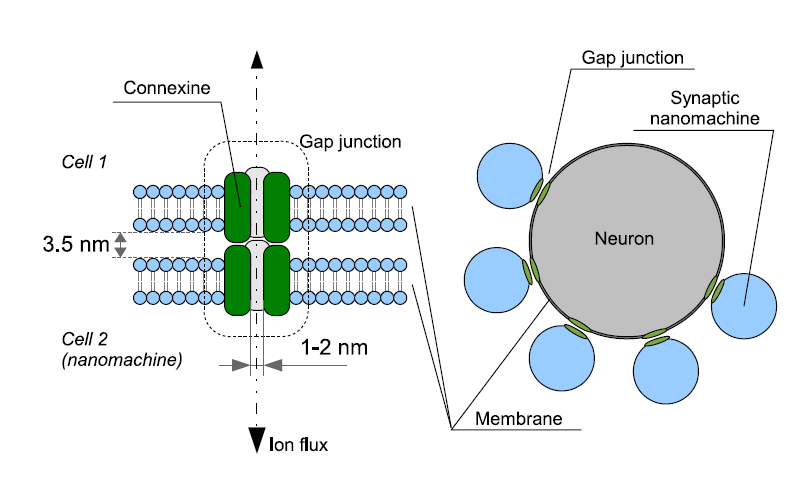
\includegraphics[width=.78\textwidth,height=.3\textheight]{Gap.png}
\caption{ Diagram of a SnM based on gap junctions. The neuronal membrane is in contact with each SnM, establishing additional connexone channels which allow the flow of ions and currents [4].}
\label{new_1}
\end{figure}


%%%%%%%%%%%%%%%%%%%%%%%%%%%%%%%%%%%%%%%%%%%%%%%%%%%%%%%%%

\clearpage
\noindent
\begin{longtable}{|p{0.975\textwidth}|}
\hline \hline
\Centering
\cellcolor{gray!45}
\textbf{Reviewer 4} \\
\hline \hline
\RaggedRight
\cellcolor{gray!15}
\textbf{\noindent Comment 1:} ``The description of  ``unhealthy neuron'' or ``neurons that have lost their ability to communicate'' and the nano-machines to connect them seems to provide a possible future application to the communication channel model proposed. What the manuscript is not fully analyzing in the opinion of this reviewer is exactly how the nano-machines could utilize this model from an engineering perspective. If this connection is not considered to be the focus and therefore was not researched, then the consideration should be made to remove the concept of nano-machines from the ``System Model'' section (and subsequent sections) and use it merely for motivating the model.''\\
\hline
\end{longtable}
\vspace*{-1\baselineskip}
\noindent \textbf{Response:\\}
We would like to thank the reviewer for careful and thorough reading of our manuscript and for
the thoughtful comments and constructive suggestions, which helped us to improve
the quality of this manuscript. We hope that the modifications that we have made to the manuscript, and the
responses that we have provided herein will alleviate the reviewer concerns.

In recent years, engineering applications of nano-technology have also been investigated with increasing interest
for the design of bio-inspired intelligent nano-devices or nano-machines connected in a network. In this manuscript, we considered the concept of nano-machines in the proposed system model according to the reported efforts to interface the neuron's body
with synthetic nano-scale materials in the literature. We provide a brief explanation in the following. We refer to the following list of references in our explanation in this comment:


\clearpage
\begin{longtable}{|p{0.975\textwidth}|}
\hline \hline
\RaggedRight
\cellcolor{green!10}
[1] F. Patolsky, B. P. Timko, G. Yu, Y. Fang, A. B. Greytak, G. Zheng, and C. M. Lieber, ``Detection, stimulation, and inhibition of neuronal signals with high-density nanowire transistor arrays,'' Science, vol. 313, no. 5790, pp. 1100-1104, 2006.

[2] N. Sakai, J. Mareda, and S. Matile, ``Ion channels and pores, made from scratch,'' Molecular BioSyst., vol. 3, pp. 658-666, 2007.

[3] P. Gorostiza and E. Isacoff, ``Optical switches and triggers for the manipulation of ion channels and pores,'' Molecular BioSyst., vol. 3, pp. 686-704, 2007.

[4] Mesiti, Fabio, and Ilangko Balasingham. ``Nanomachine-to-neuron communication interfaces for neuronal stimulation at nanoscale.'', IEEE Journal on Selected Areas in Communications, vol. 31, no. 12, pp. 695-704, 2013.

[5] N. Rouach, E. Avignone, W. Même, A. Koulakoff, L. Venance, F. Blomstrand, and C. Giaume, ``Gap junctions and connexin expression in the normal and pathological central nervous system,'' Biology Cell, vol. 94, no. 7-8, pp. 457-475, 2002.

[6] J. Hjorth, K. T. Blackwell, and J. Hellgren Kotaleski, ``Gap junctions between striatal fast-spiking interneurons regulate spiking activity and synchronization as a function of cortical activity'', J. Neuroscience, vol. 29, no. 16, pp. 5276-5286, 2009.

[7] R. D. Traub, M. A. Whittington, E. H. Buhl, F. E. N. LeBeau, A. Bibbig, S. Boyd, H. Cross, and T. Baldeweg, ``A possible role for gap junctions in generation of very fast EEG oscillations preceding the onset of, and perhaps initiating, seizures,'' Epilepsia, vol. 42, no. 2, pp. 153-170, 2001.
\\
\hline
\end{longtable}


\clearpage
In [1], the authors described the successful attempt to interface nano-wire (NW) FET transistors (SiNW-neurons) with soma, dendrites and axon, allowing high precision measurement and
stimulation with an array of 50 NW connections per neuron. The synthesis of ion channels and pores, assembled artificially by chemical composition were reported in [2], whereas synthetic nano-scale actuators (nano-toggles, nano-keys and nano-tweezers) to manipulate ion channels were proposed in [3].
Hence, the advances in the molecular manipulation of the matter can allow the fabrication of bio-inspired SnM interfaces.
Upon these considerations and the available nano-technology, the authors in [4] identified a set of possible SnM interface implementations. We employed one type of these interfaces in our system model according to [4] which is denoted as Gap Junction Interface.


\textbf{Gap Junction Interface [4]}:

With gap junctions, two cellular membranes in direct contact are separated by only 3 nm and for each side, clusters of \textit{connexine} (Cx36) proteins [5], combine to form a channel with diameter 1-2 nm, the \textit{connexine}, allowing bidirectional flows of ions (currents) between cells. Synthetic connexines assembled \textit{in-situ} by SnMs could allow the opening of additional ion channels on the membrane, enhancing the neuronal activity. In the following figure [4], a sample scenario with multiple SnMs attached to the target neuron is depicted. This method is motivated and supported by neuro-scientific studies [6], [7] reporting the important role of gap junctions in \textit{oscillatory behaviors} and \textit{synchronization} phenomena between neurons.

\begin{figure}[H]
\centering
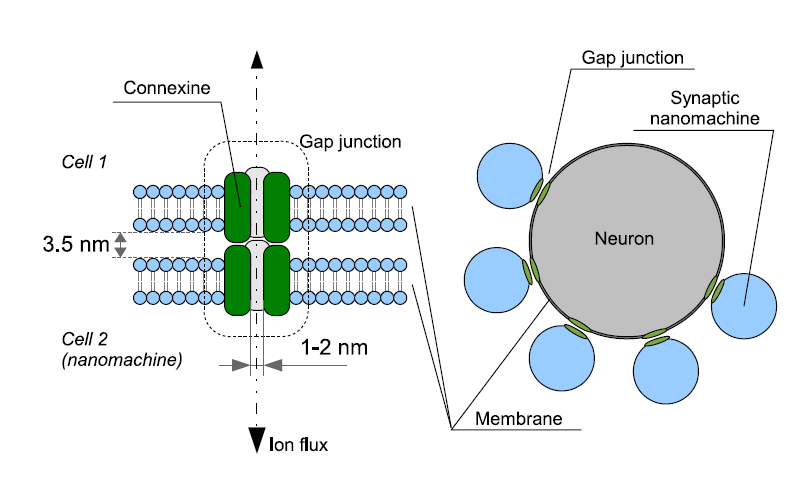
\includegraphics[width=.78\textwidth,height=.3\textheight]{Gap.png}
\caption{ Diagram of a SnM based on gap junctions. The neuronal membrane is in contact with each SnM, establishing additional connexone channels which allow the flow of ions and currents [4].}
\label{new_1}
\end{figure}










\end{document}


